\documentclass[a4paper]{article}

\usepackage{graphicx, subfigure}          % To handle figures

\usepackage{amsmath}           % Defines certain mathematical symbols
%\usepackage{psfrag}            % Inserts LaTeX text into figures (does not work with PDFLatex)
\usepackage{url}               % To typeset email addresses and URLs
\usepackage[latin1]{inputenc}  % Makes sure that all Swedish characters
                               % work
%\usepackage[swedish]{babel}    % If you want to write in Swedish.

%\addtolength{\topmargin}{-25mm}% Decrease the top margin by 25mm
%\addtolength{\textheight}{25mm}% Increase the text height by the
                               % same amount

\usepackage[margin={2.5cm,2cm}]{geometry}
\usepackage{lipsum}
%\usepackage{multicol}
%\usepackage{tikz}
%\usetikzlibrary{dsp,chains}
\usepackage{listings}

\renewcommand*\sfdefault{lmssq}
\renewcommand*\familydefault{\sfdefault} %% Only if the base font of the document is to be sans serif
\usepackage[T1]{fontenc}

\DeclareMathAlphabet{\mathpzc}{OT1}{pzc}{m}{it}
\newcommand{\z}{\mathpzc{z}}


\begin{document}

\title{Advanced Wireless Communications: Algorithms and Architectures  \\ }
\author{Raffael Fabian Tschui}
\date{March 13, 2015 \\ EPFL} % If you don't want todays date.

\maketitle

%\begin{multicols*}{2}
  
\section{DSSS \& CDMA}
\subsection{Spreading sequence}

To spread the energy of a symbol over a wider bandwidth, it is multiplied with a so called spreading sequence, which is then again removed by using a correlator at the receiver side Commonly, Barker codes are used for this and the given sequence in this lab was [1 1 1 -1 -1 1 -1]. The exact same performance can be obtained when taking the same sequence with all the signs inverted, e.g. [-1 -1 -1 1 1 -1 1 ]. Obviously, this sequence has exactly the same correlation properties which would be the criterion for equal performance in a transmission system.

The length of the spreading sequence influences the performance significantly. Of course, one would assume that a longer sequence gives better performance, as the signal is spread over a wider bandwidth. As a reminder, the bandwidth is approximately proportional to the chiprate:

\begin{equation}
B_{c} \approx 1/T_{c} = G/T_{s}= G B
\end{equation}

where $G$ is the spreading sequence length, $B_{c}$ the chip bandwidth and $B$ the original bandwidth. The hypothesis can be confirmed when looking at figure \ref{fig:spreadlength} in which the performance of different sequence lengths have been simulated.

\begin{figure}[htbp]
\begin{center}
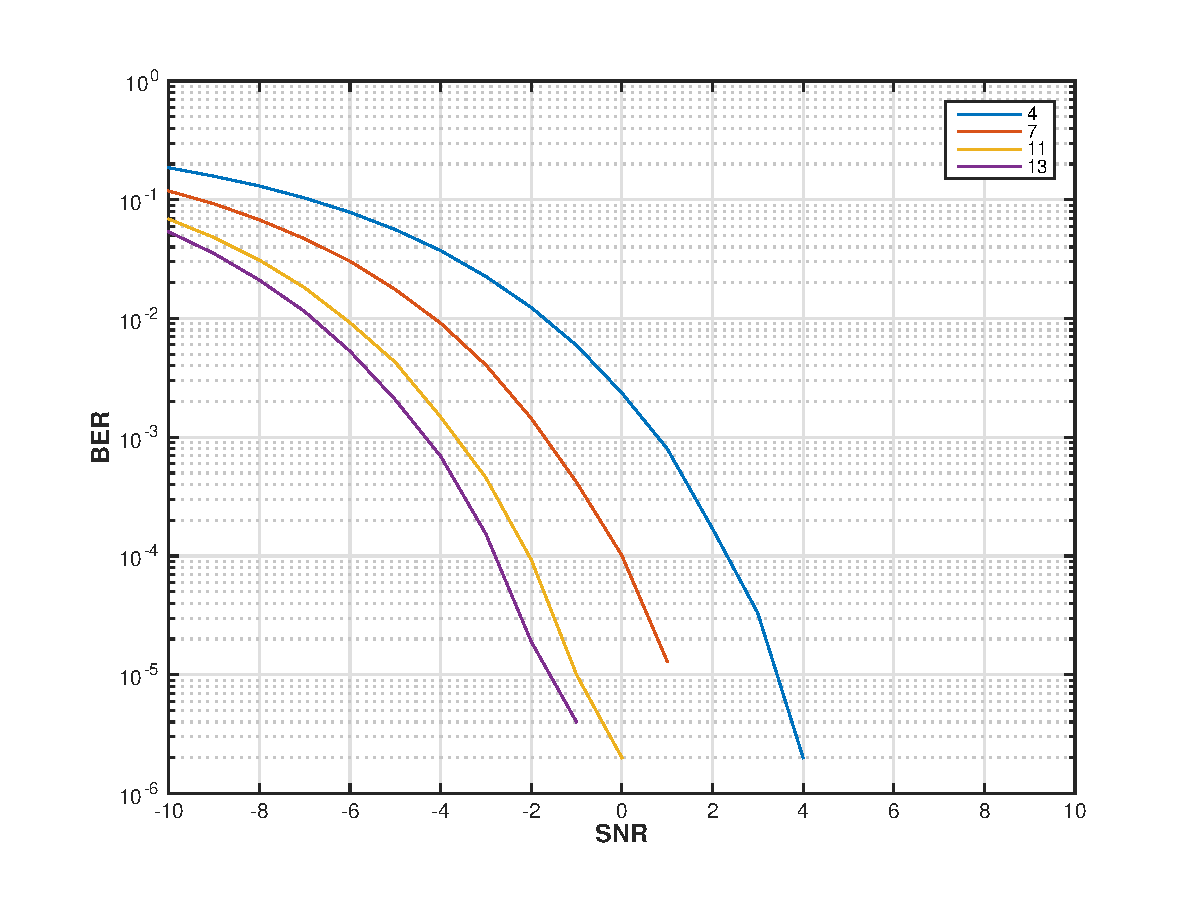
\includegraphics[width=.6\textwidth]{img1/spreading_lengths.eps}
\caption{BER plot for different spreading sequence lengths}
\label{fig:spreadlength}
\end{center}
\end{figure}

However, spreading a sequence over a wider bandwidth also means that a larger portion of the noise floor is distorting the signal. Therefore, the curves need to be SNR-adjusted and the resulting graph is depicted in figure \ref{fig:compensated}. Now we see all the curves lying on top of each other, meaning that we don't actually gain anything in performance when increasing the sequence length, if we do a fair comparison.

\begin{figure}[htbp]
\begin{center}
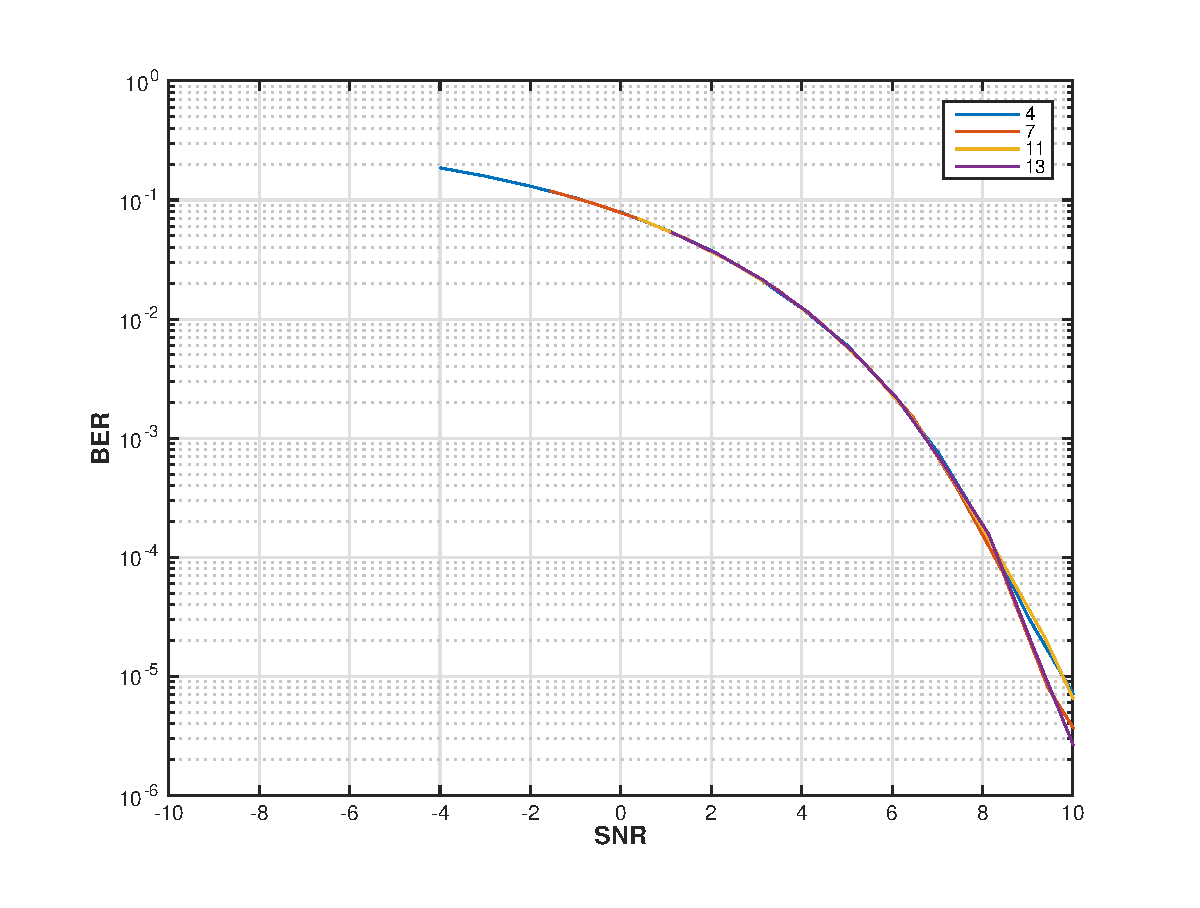
\includegraphics[width=.6\textwidth]{img1/compensated.eps}
\caption{SNR compensated BER plot}
\label{fig:compensated}
\end{center}
\end{figure}

\subsection{Rake Receiver and multipath environment}

To simulate a multipath environment, the channel was modelled with a FIR of length>1. To compensate for this kind of channel, one has to get rid of intersymbol (or ``inter-chip'') interference. Figure \ref{fig:rakefinger} taken from the course illustrates this very well. The received signal is correlated with a delayed version of the chip sequence and then weighted with the complex conjugate the channel coefficient (that we assume to be known - in practice this would be done through channel estimation). The outputs of all the fingers are then summed up to reconstruct the initial information.

\begin{figure}[htbp]
\begin{center}
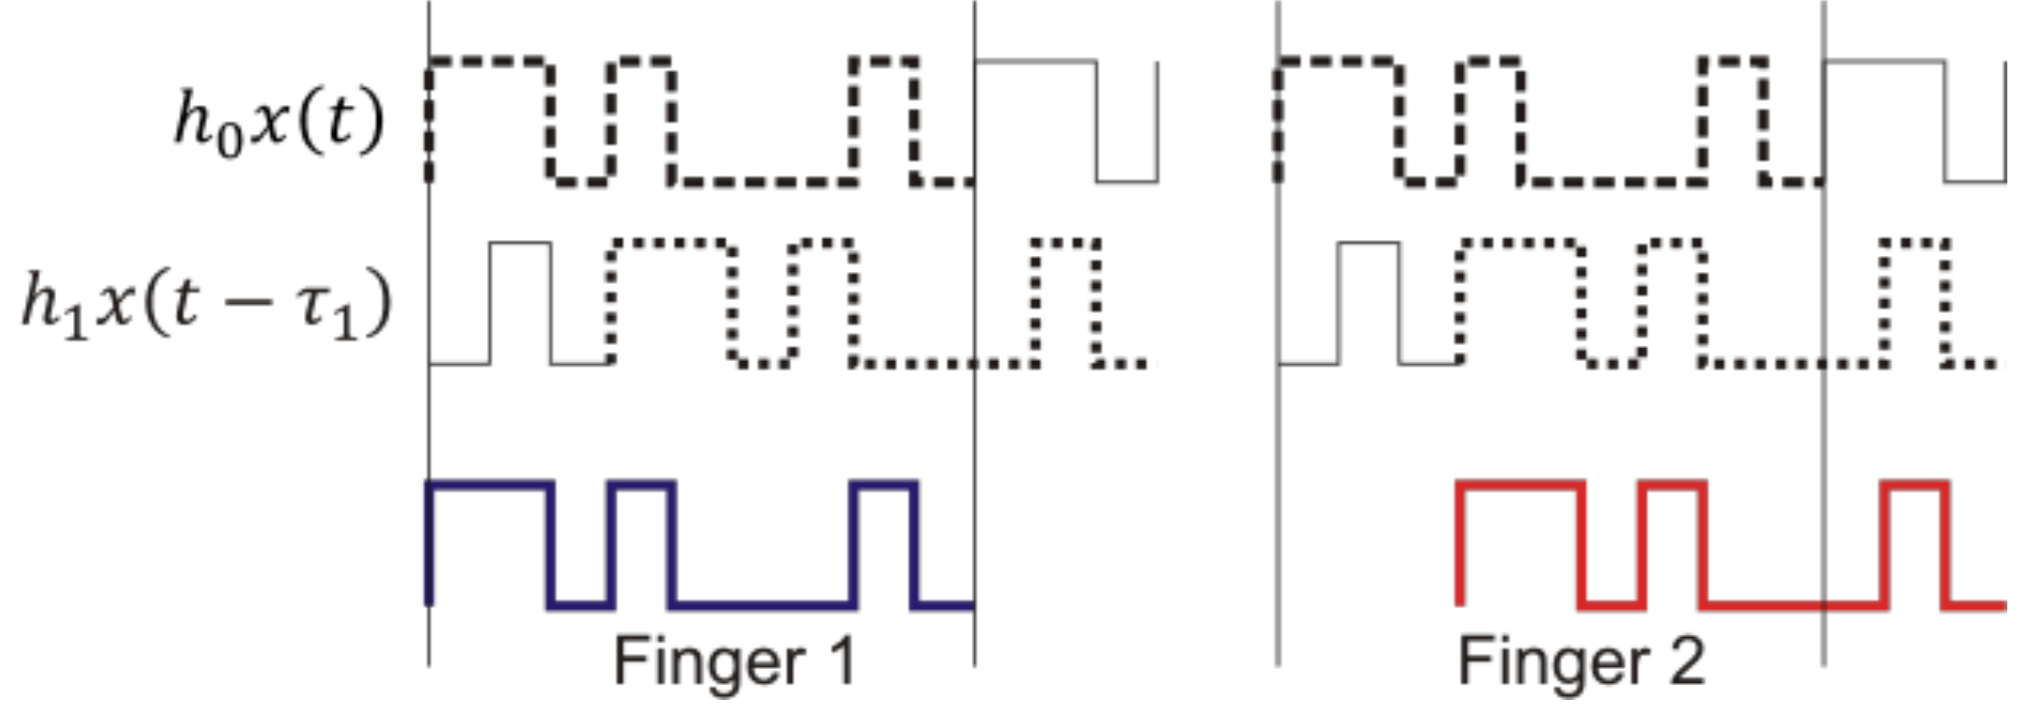
\includegraphics[width=.6\textwidth]{img1/rakefinger.png}
\caption{The different fingers of a rake receiver correlate the spreading sequence with delayed versions of the received signal to compensate for the multipath channel.}
\label{fig:rakefinger}
\end{center}
\end{figure}

Figure \ref{fig:rake} shows the performance of the MATLAB implemented rake receiver for a channel length of 3 taps. Note that the SNR decreases when using more fingers, which is explained through the fact that more information is extracted from the received signal.

\begin{figure}[htbp]
\begin{center}
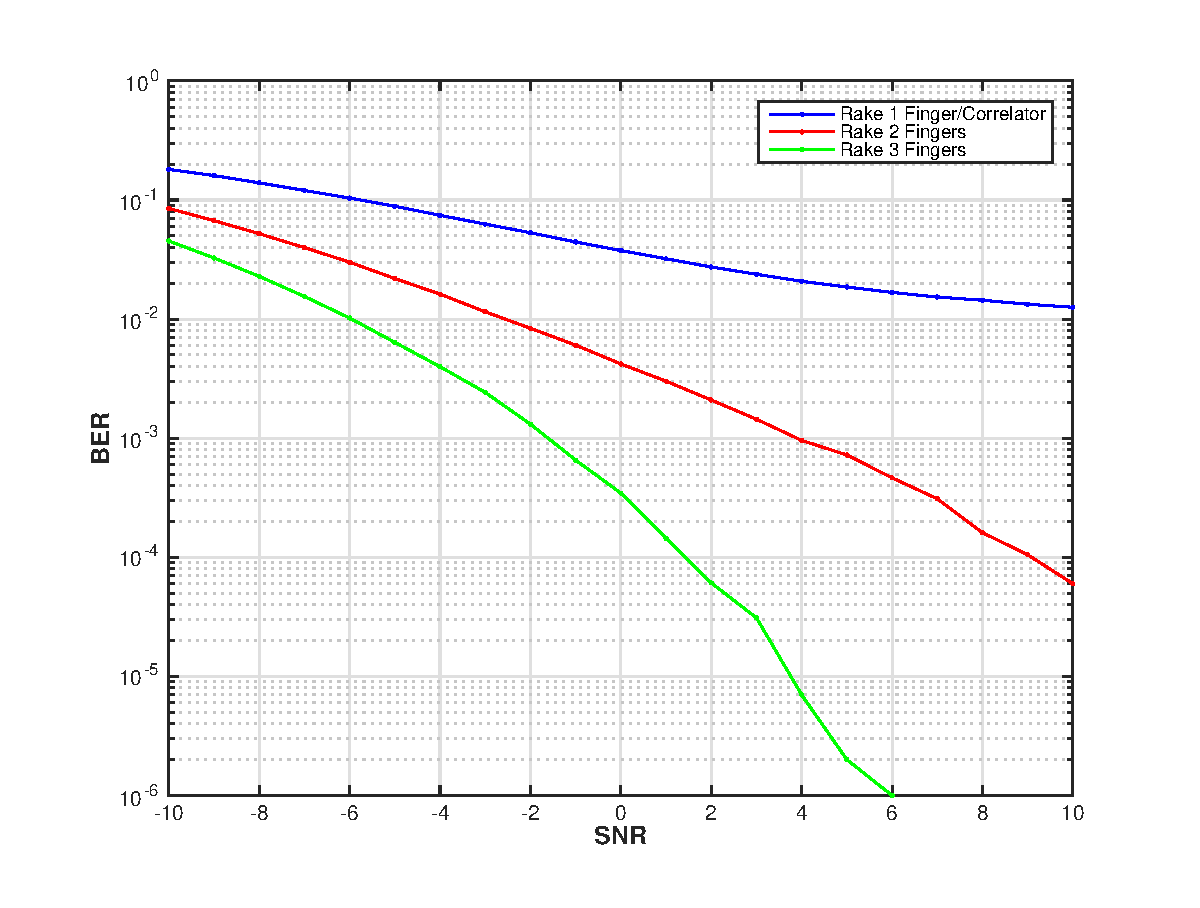
\includegraphics[width=.6\textwidth]{img1/rake.eps}
\caption{Rake receiver performance with different number of fingers.}
\label{fig:rake}
\end{center}
\end{figure}

\newpage 

\subsection{CDMA broadcast scenario}
CDMA stands for code division multiple access and it is a way to transmit information for multiple users at the same time (or inverse). Each user has therefore its ``personal'' spreading sequence that is orthogonal to the one of other users, so no user signal will disturb the other due to this orthogonality. A good choice are the so called Hadamard codes. 

They present, however, bad autocorrelation properties. In a case where we have multipath, this is therefore not very helpful and a rake receiver wouldn't perform as expected. Therefore, the signal is after spreading again multiplied with a Barker code. This \textit{doesn't} increase the spreading factor, but it gives the transmitted signal a good autocorrelation property. As a plus, different base stations can now use different Barker code sequences, so they won't interfere with each other.

Figure \ref{fig:1b2} shows the simulation result of the implemented receiver scheme for 1, 2 and 4 users in an AWGN environment. As can be seen, the overall averaged BER stays the same, even when increasing the number of users. This is thanks to the orthogonality of the Hadamard matrix.

\begin{figure}[htbp]
\begin{center}
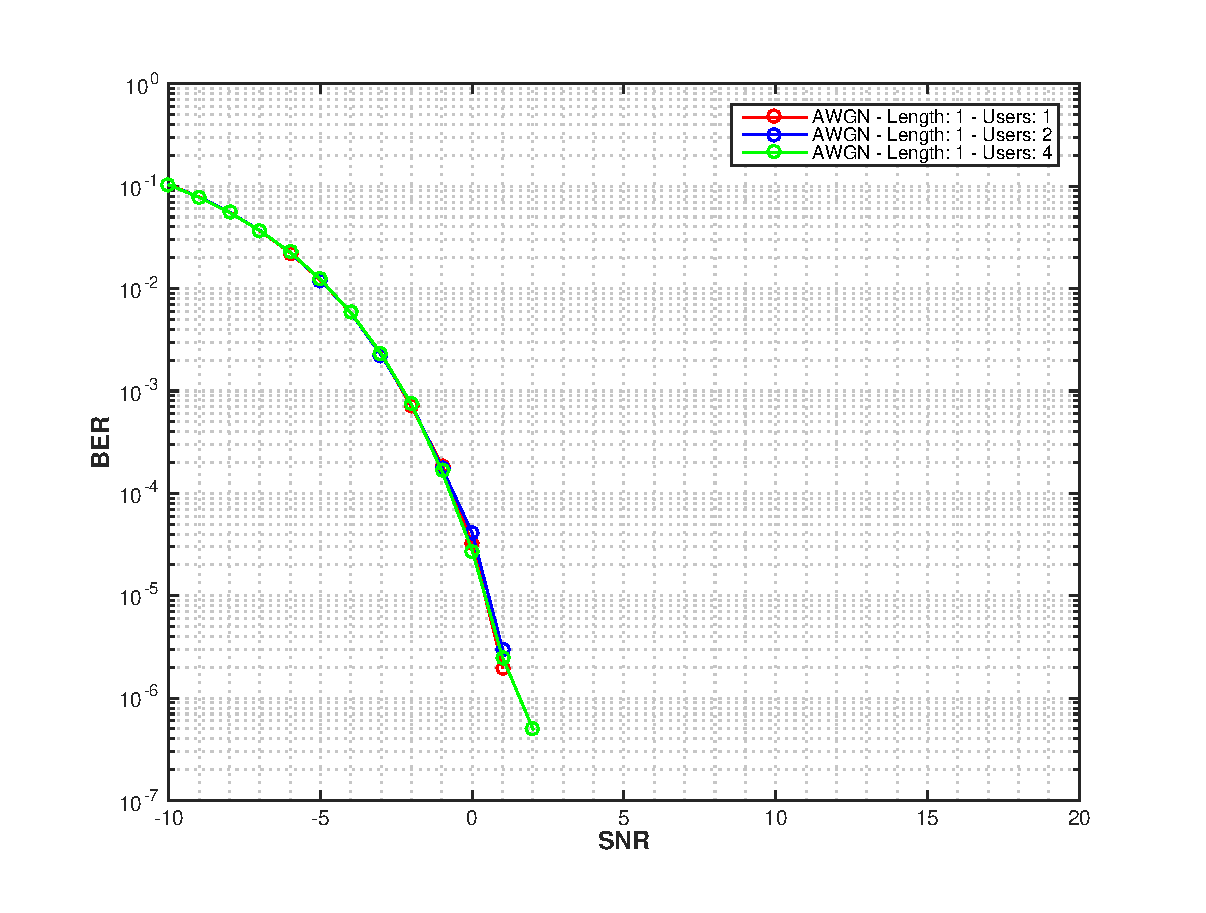
\includegraphics[width=.6\textwidth]{img1/1b2.eps}
\caption{Testing CDMA receiver for 1, 2 and 4 users with AWGN channel.}
\label{fig:1b2}
\end{center}
\end{figure}


Figures \ref{fig:1b3} and \ref{fig:1b4} show the same (rake) receiver performing when having a fading and multipath channel respectively. Compared to the AWGN case, the SNR became already much worse in the fading channel, however increasing the number of users doesn't affect this.


\begin{figure}[htbp]
\begin{center}
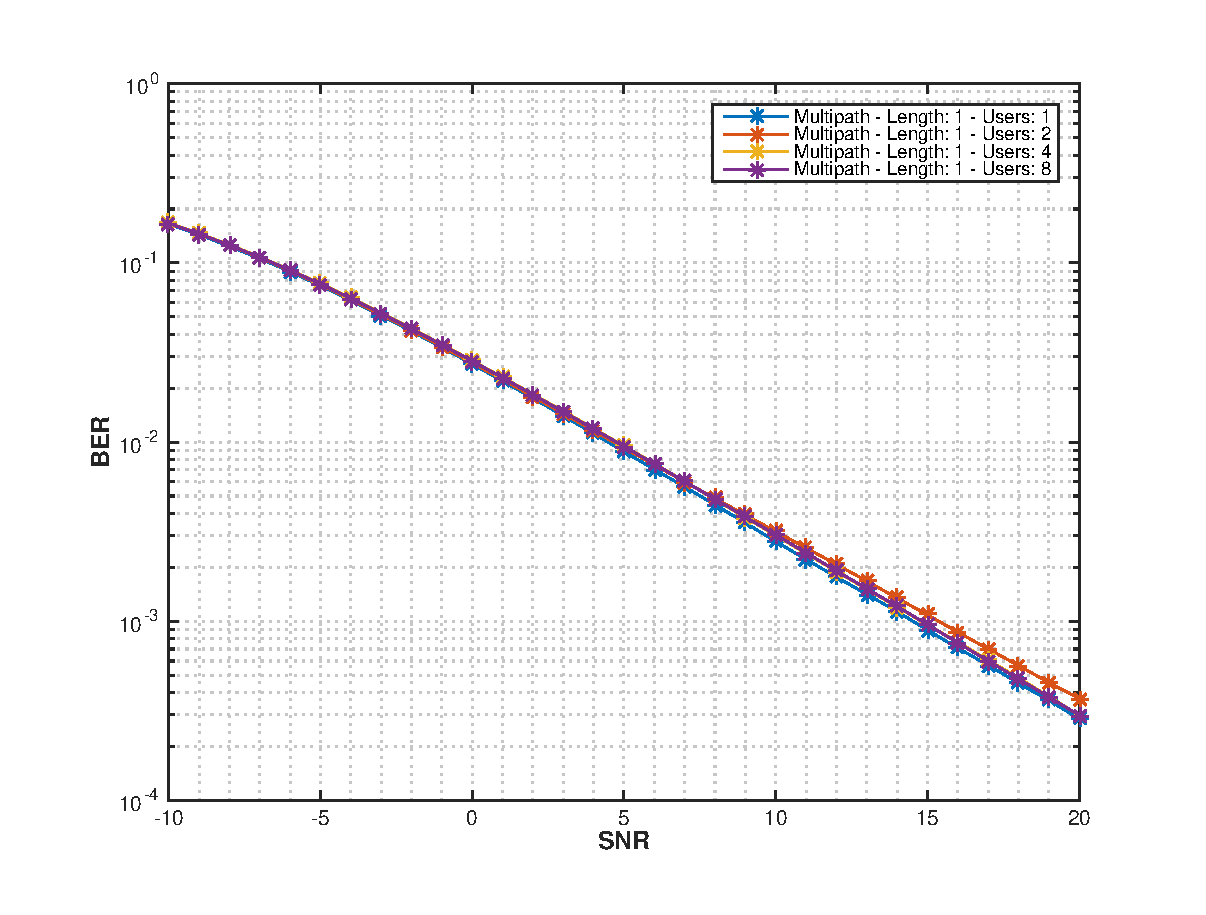
\includegraphics[width=.6\textwidth]{img1/1b3.eps}
\caption{CDMA receiver for 1, 2, 4 and 8 users while having fading.}
\label{fig:1b3}
\end{center}
\end{figure}


\begin{figure}[htbp]
\begin{center}
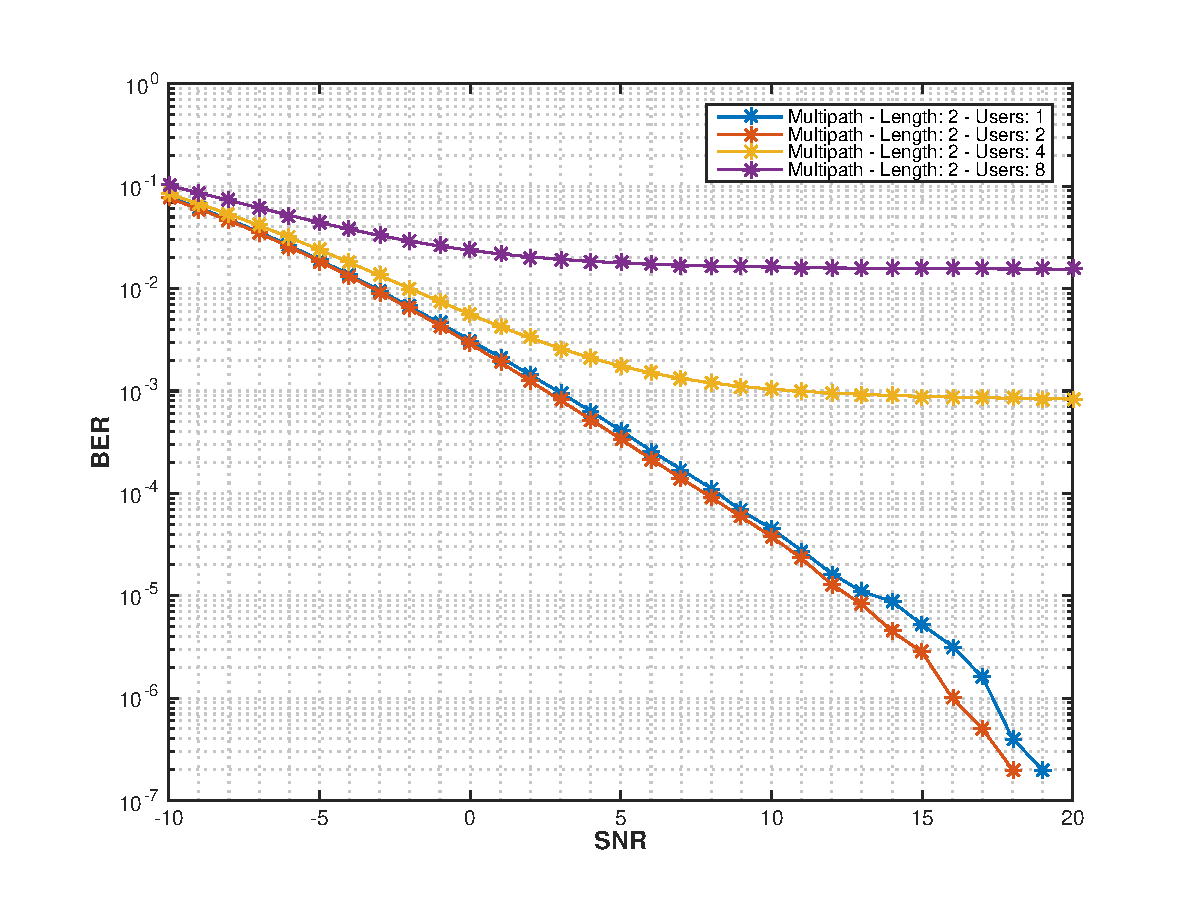
\includegraphics[width=.6\textwidth]{img1/1b4.eps}
\caption{CDMA receiver for 1, 2, 4 and 8 users in a fading multipath environment.}
\label{fig:1b4}
\end{center}
\end{figure}

The multipath case is even worse: Now the number of users have a great influence on the performance and the BER seems to converge to a fixed value even though the SNR increases.

In figure \ref{fig:channellength} the channel length was increased. Surprisingly, for low SNR, the BER decreases when the channel gets longer. Only the asymptote for 4 or more users has a higher BER value for more channel taps. This is quite non-intuitive and might be related to the choice of the spread-sequence (Hadamard codes) and intersymbol interference due to their bad autocorrelation properties.

\begin{figure}
    \centering
        \subfigure[2 taps]{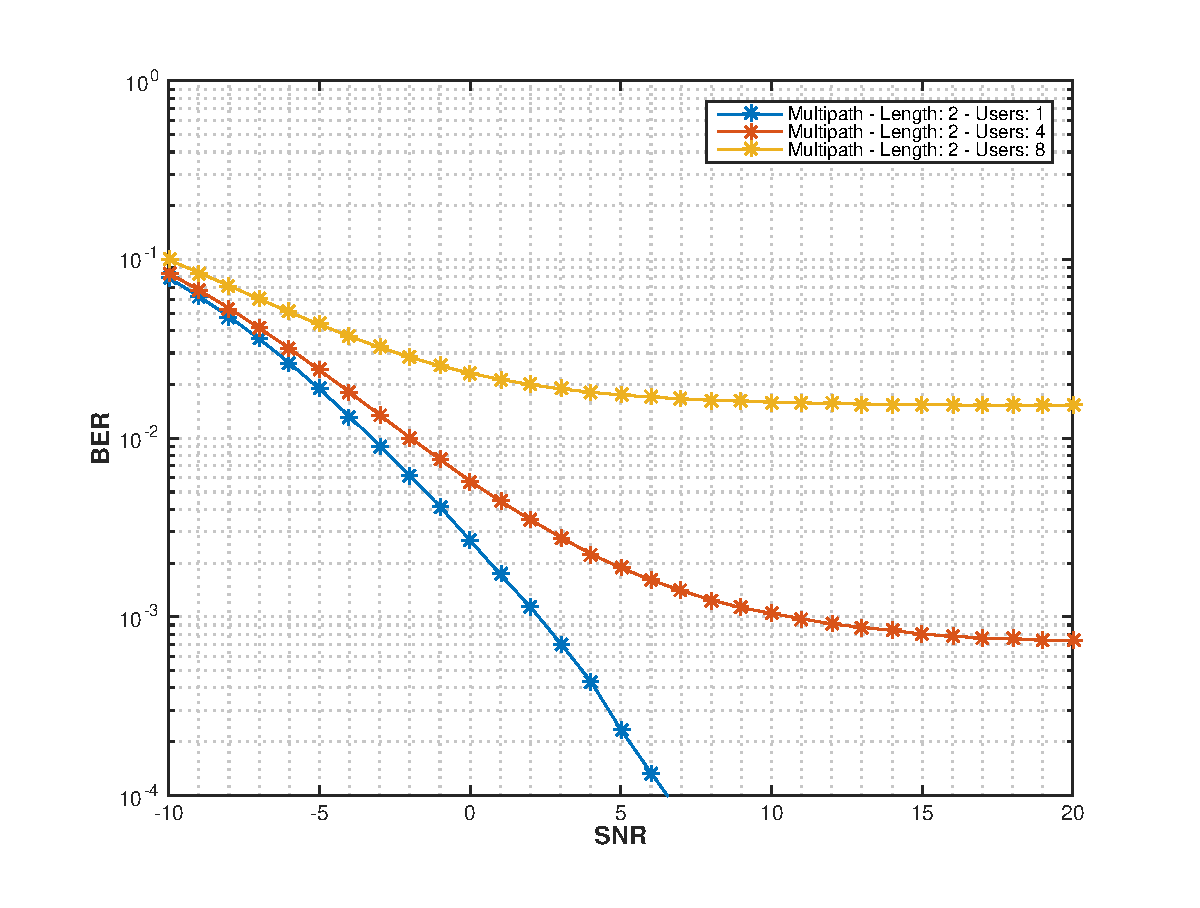
\includegraphics[width=0.3\textwidth]{img1/mp2.eps}}
        \subfigure[3 taps]{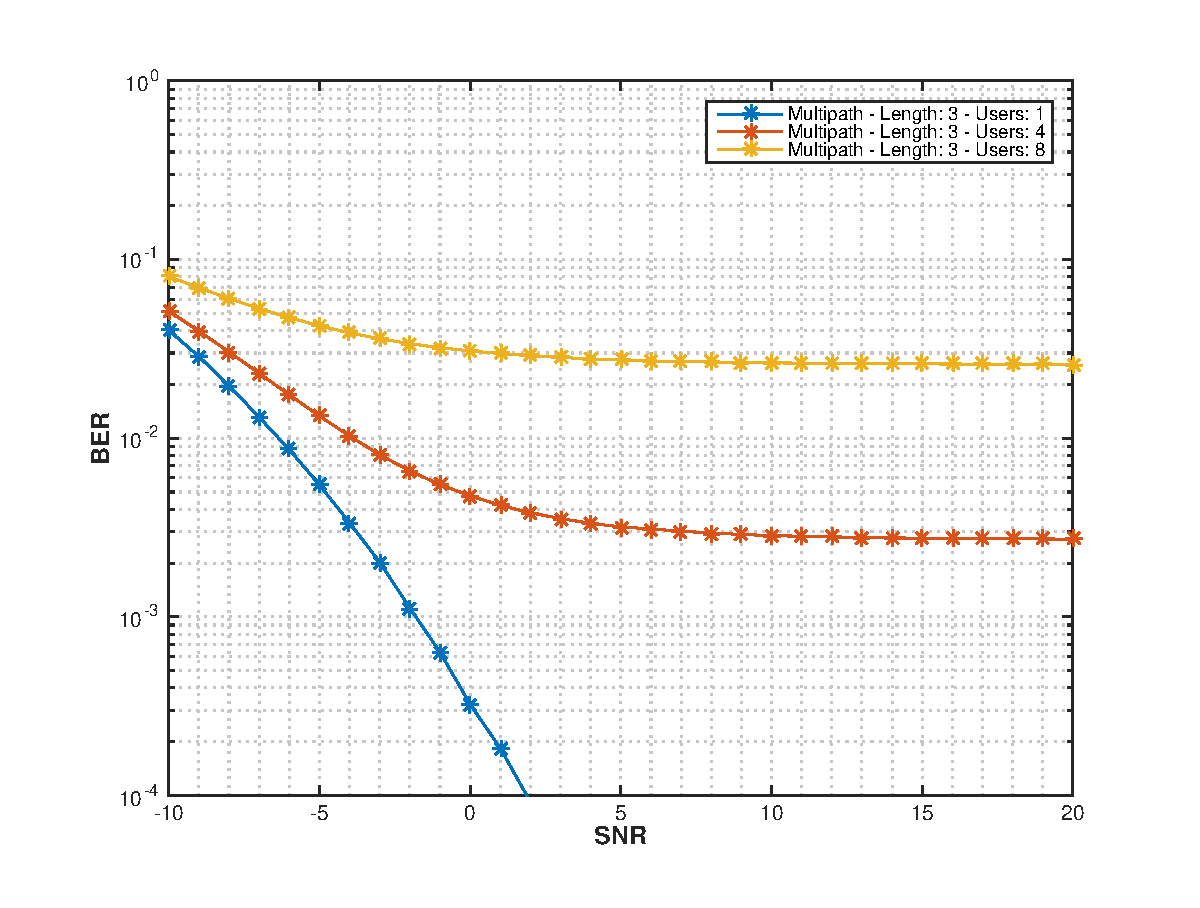
\includegraphics[width=0.3\textwidth]{img1/mp3.eps}}
        \subfigure[4 taps]{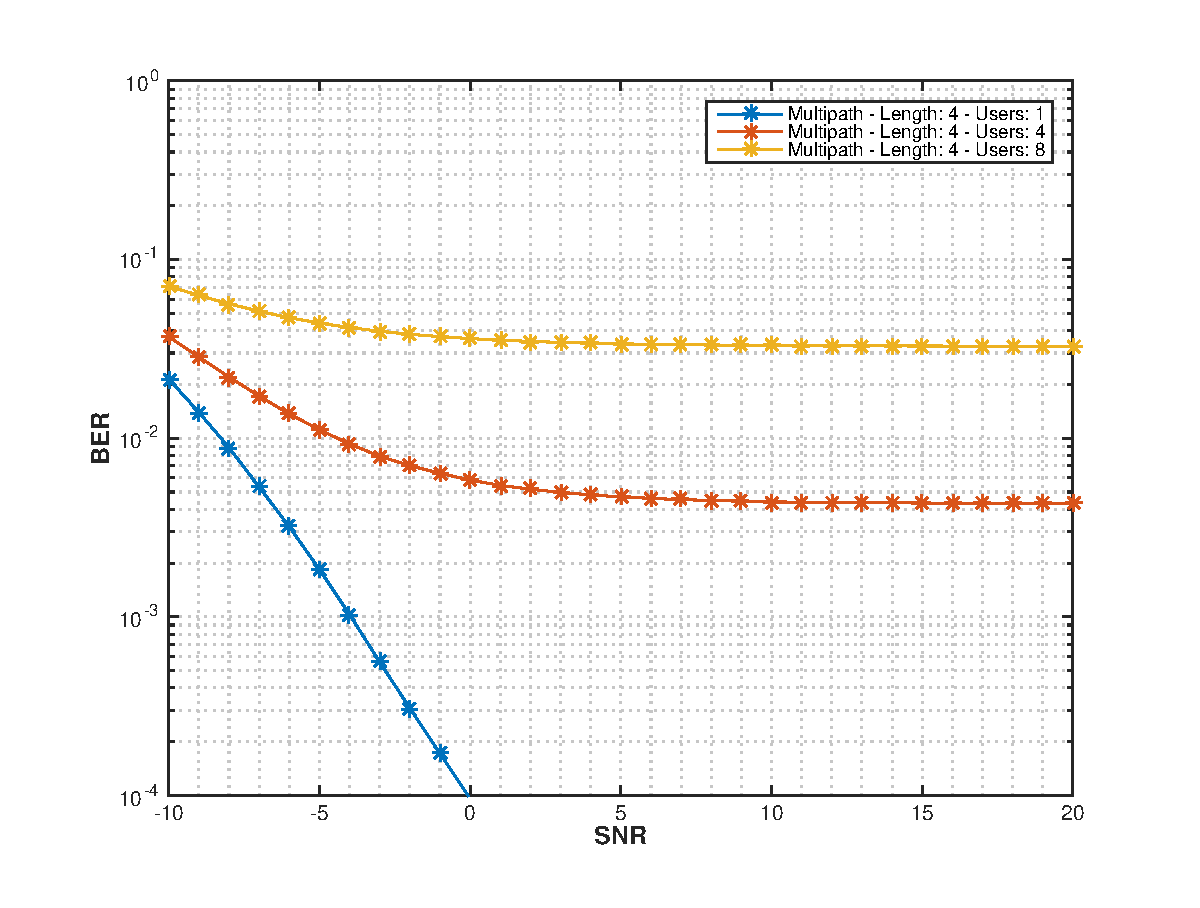
\includegraphics[width=0.3\textwidth]{img1/mp4.eps}}
        
      \caption{CDMA receiver for 1, 4 and 8 users in a fading multipath environment with different channel lengths (number of taps).}
    \label{fig:channellength}
    \end{figure}


\end{document}